\documentclass{article}

\usepackage[T1]{fontenc}
\usepackage[utf8]{inputenc}
\usepackage[polish]{babel}
\usepackage{amsmath, amsfonts}
%\usepackage{amssymb}
\usepackage{mathtools}
\usepackage{xfrac}
\usepackage{textcomp}
\usepackage{graphicx}
\graphicspath{{.}}
\usepackage[nofoot,hdivide={2cm,*,2cm},vdivide={2cm,*,2cm}]{geometry}

\author{Jacek Długopolski}
\title{Kolokwium 1}
\date{\today}

\begin{document}
\maketitle

\section*{Zadanie 1}
\begin{itemize}
\item$\rho \frac{D\textbf{u}}{Dt} = \rho \big( \frac{\partial\textbf{u}}{\partial t} + \textbf{u} \cdot \nabla \textbf{u})=-\nabla \overline{p}+\nabla\cdot\{\mu(\nabla \textbf{u}+(\nabla \textbf{u})^\text{T}-\frac{2}{3}(\nabla\cdot \textbf{u})\textbf{I}\}+ \rho\textbf{g}$

\item$\overline{f}(\xi)=\int_{-\infty}^{\infty} f(x)$ $e^{-2\pi ix\xi}dx$

\item$\mathbb{P}(\hat{X}_{n}-z_{1-\frac{\alpha}{2}}\frac{\sigma}{\sqrt{n}}\le \mathbb{E}X \le\hat{X}_{n}+z_{1-\frac{\alpha}{2}}\frac{\sigma}{\sqrt{n}})\approx 1 -\alpha$

\item$\begin{bmatrix}1&2\\3&4\end{bmatrix} \otimes\begin{bmatrix}0&5\\6&7\end{bmatrix}=\begin{bmatrix}1\begin{bmatrix}0&5\\6&7\end{bmatrix}&
2\begin{bmatrix}0&5\\6&7\end{bmatrix}\\3\begin{bmatrix}0&5\\6&7\end{bmatrix}&4\begin{bmatrix}0&5\\6&7\end{bmatrix} \end{bmatrix}=
\begin{bmatrix}0&5&0&10\\6&7&12&14\\0&15&0&20\\18&21&24&28\end{bmatrix}$
\end{itemize}

\section*{Zadanie 2}
\begin{enumerate}
 \item Generuję lokalnie dwa klucze ssh poleceniem: 
 \begin{verbatim}
    ssh-keygen
 \end{verbatim}
 Polecenie ssh-keygen wywołane bez argumentów generuje klucz RSA.\\
 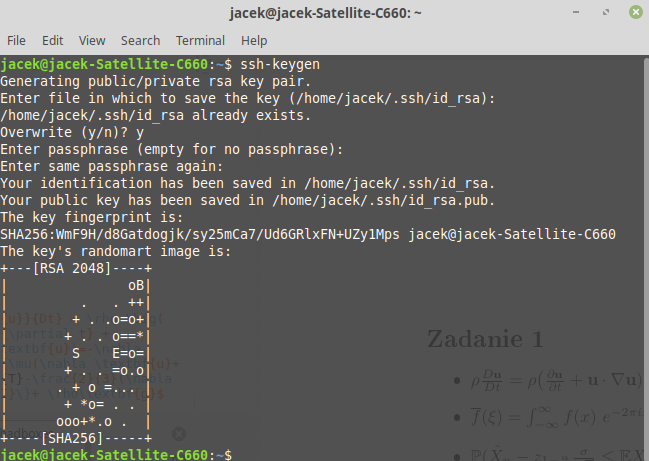
\includegraphics[scale=0.4]{ssh-keygen2.png}
 \item Przenoszę klucz na zdalny serwer używając polecenia:
 \begin{verbatim}
  ssh-copy-id -i ~/.ssh/id_rsa.pub d324130@pwi.ii.uni.wroc.pl
 \end{verbatim}
 -i identityfile Use only the key(s) contained in identityfile (rather than looking for identities via ssh-add(1) or in the defaultIDfile)\cite{sshcopy}
 \\
 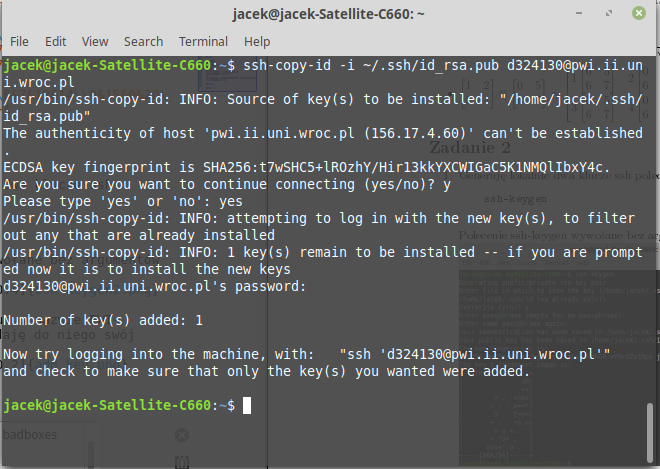
\includegraphics[scale=0.4]{ssh-copy-id2.png}

 \item Tworzę repozytorium o nazwie PWI-sprawdzian-d324130 i dodaję do niego swój wygenerowany klucz:\\
 
 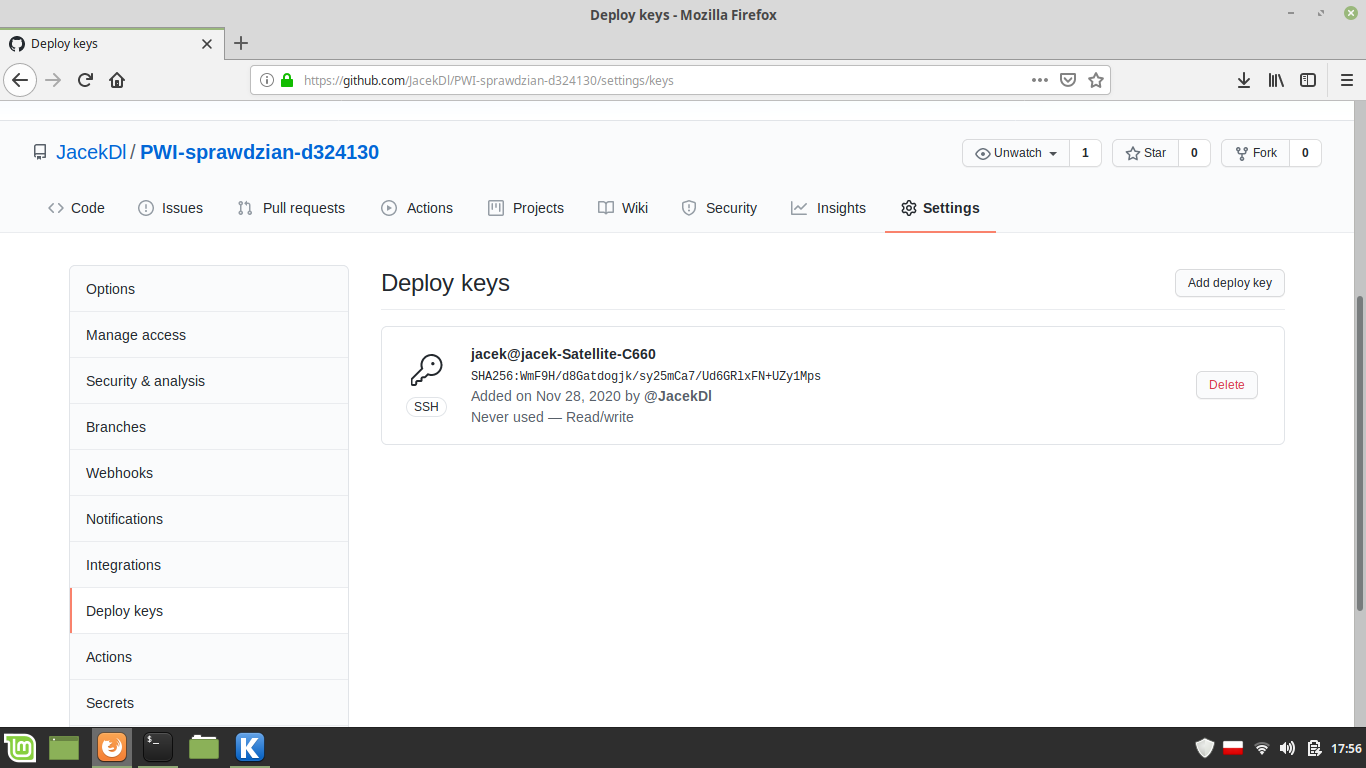
\includegraphics[scale=0.2]{add_key.png}
 \item Tworzę plik konfiguracyjny dla ssh, który umożliwia logowanie na serwer za pomocą polecenia:
 \begin{verbatim}
  ssh pwi-sprawdzian
 \end{verbatim}
 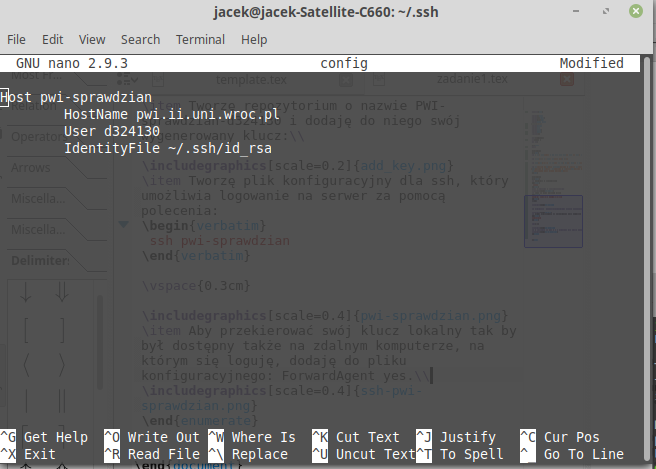
\includegraphics[scale=0.4]{config.png}
 \vspace{0.3cm}
 
 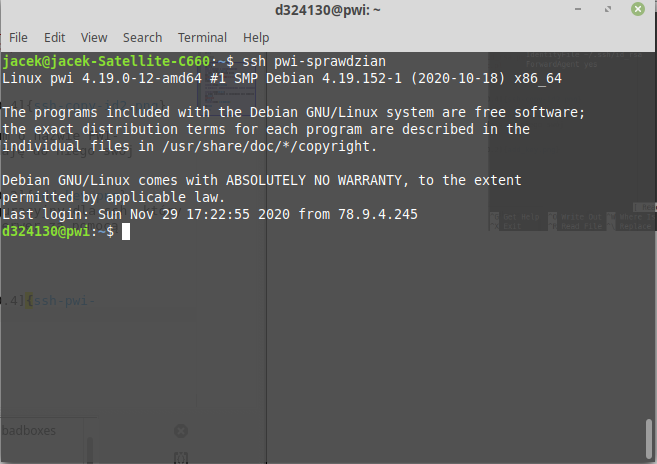
\includegraphics[scale=0.4]{pwi-sprawdzian.png}
 \item Aby przekierować swój klucz lokalny tak by był dostępny także na zdalnym komputerze, na którym się loguję, dodaję do pliku konfiguracyjnego: ForwardAgent yes\cite{forward}\\
 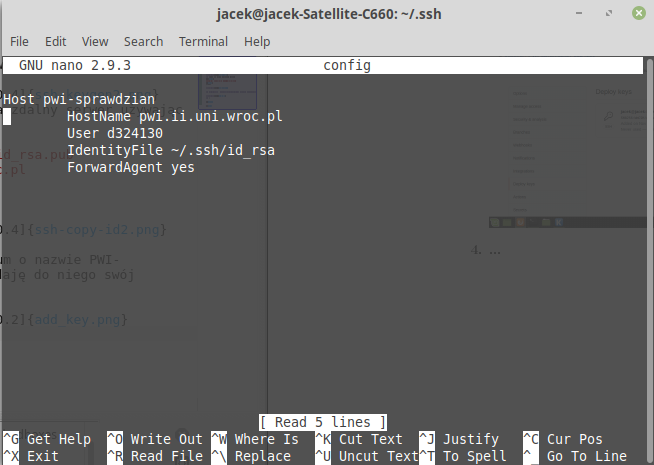
\includegraphics[scale=0.4]{ssh-pwi-sprawdzian.png}
 \vspace{0.3cm}
 \\Rozwiązanie polegające na wygenerowaniu kolejnego klucza jest 'brzydkie', ponieważ tworzy również klucz prywatny, który pozostaje na zdalnym komputerze.
 \end{enumerate}
 \section*{Zadanie 3}
 \begin{enumerate}
  \item Loguję się na pwi.ii.uni.wroc.pl. Klonuję repozytorium z GitHuba poleceniem:
  \begin{verbatim}
   git clone git@github.com:JacekDl/PWI-sprawdzian-d324130.git
  \end{verbatim}
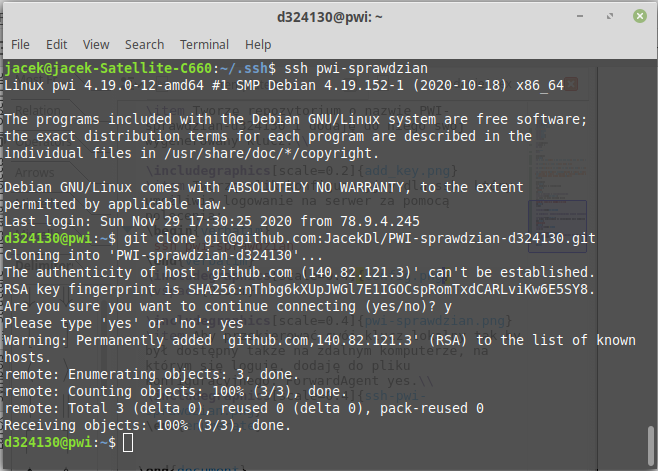
\includegraphics[scale=0.4]{gitclone.png}
\item Pobieram poleceniem wget plik ze strony:
\begin{verbatim}
 wget http://www.ii.uni.wroc.pl/~lisu/zadanie.tar.gz
\end{verbatim}
Następnie wypakowuję ten plik w repozytorium:
\begin{verbatim}
 tar -xf zadanie.tar.gz
\end{verbatim}
-x wyodrębnia pliki\\
-f określa nazwę pliku archiwum tar\cite{tar}\\
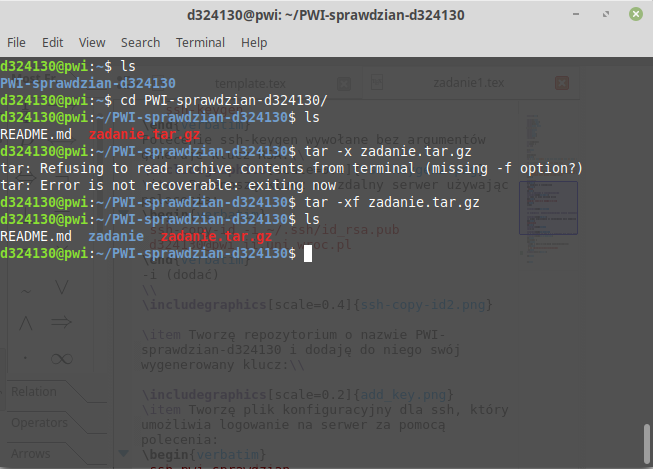
\includegraphics[scale=0.4]{tar.png}\\
I komituję zmiany:
\begin{verbatim}
 git add .
 git commit -m "Dodano pliki z archiwum tar"
\end{verbatim}
\item Wyliczam funkcję skrótu MD5 ze stringa d324130 poleceniem:
\begin{verbatim}
 echo -n "d324130" | md5sum
\end{verbatim}
-n nie dolicza znaku nowej linii na końcu napisu podanego jako argument\cite{bytefreaks}\\
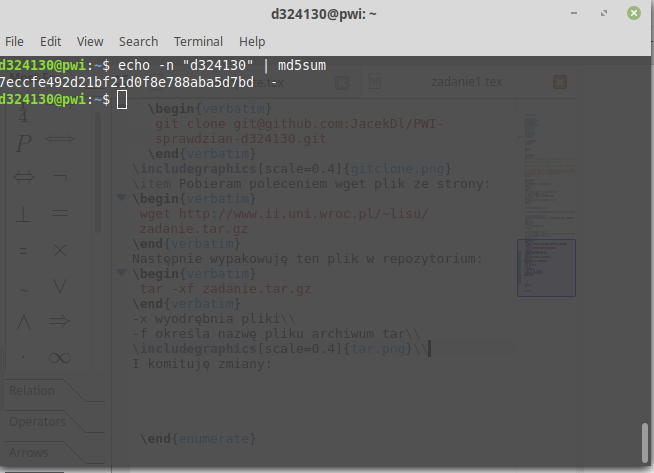
\includegraphics[scale=0.4]{md5sum.png}\\
Odnajduję w gąszczu pobranych folderów katalog:
\begin{verbatim}
 find -name "7eccfe492d21bf21d0f8e788aba5d7bd"
\end{verbatim}
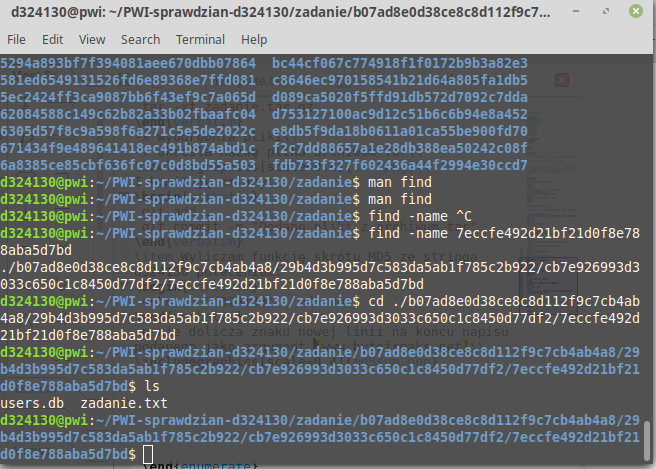
\includegraphics[scale=0.4]{find.png}\\
Następnie wykonuję polecenia z zadania:

a) Sprawdzam jaki jest procentowy stosunek użytkowników z Polski do wszystkich którym wykradziono hasła:
 \begin{verbatim}
  grep -c "Country" users.db
  grep -c "Country = POLAND" users.db 
 \end{verbatim}
 I wykorzystuję pythona do obliczeń:\\
 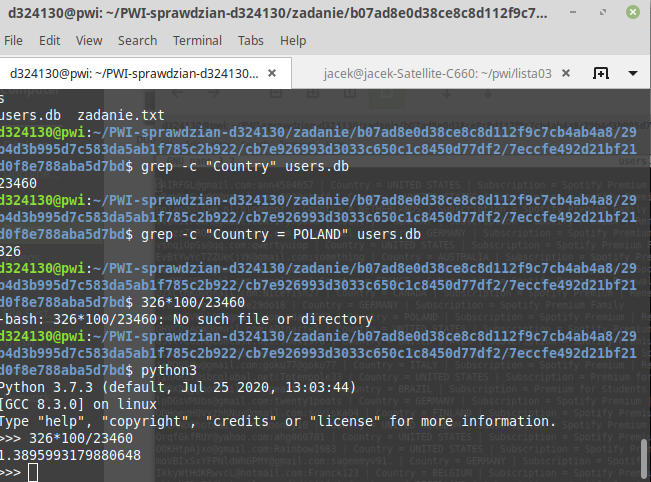
\includegraphics[scale=0.4]{zadanie.png}\\
 Wynik $\approx 1,39 \%$
 \\b) Tworzę nowy plik passwords.txt do którego zapisuję tylko hasła z users.db poleceniami:
 \begin{verbatim}
  touch passwords.txt
  sed 's/.*://' users.db > passwords.txt
  sed -i 's/|.*//' passwords.txt
 \end{verbatim}
 -i działa w miejscu - modyfikuje plik podany w komendzie\cite{sed}\\
 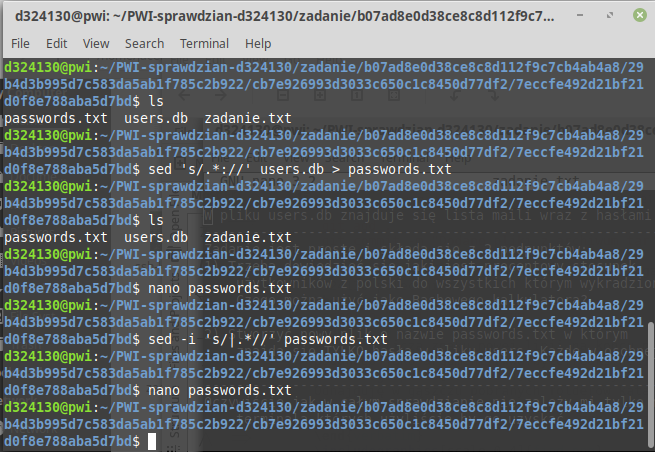
\includegraphics[scale=0.4]{passwords.png}\vspace{0.3cm}\\
 W wyniku czego otrzymuję plik zawierający tylko hasła:\\
 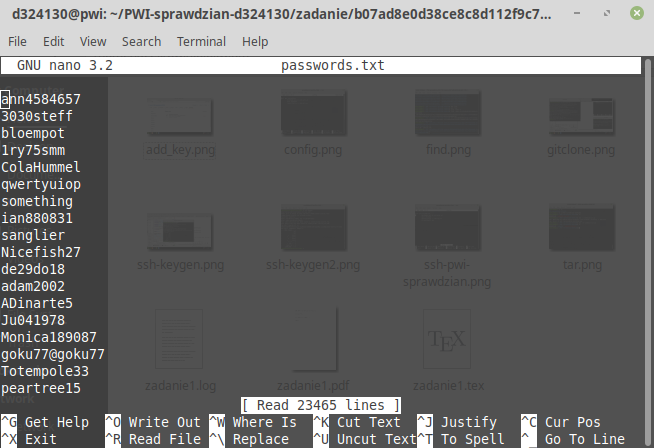
\includegraphics[scale=0.4]{pass.png}

\section*{Zadanie 4}
Kompiluję dwukrotnie plik zadanie1.tex, w wyniku czego otrzymuję plik zadanie1.pdf:
\begin{verbatim}
 pdflatex zadanie1.tex
\end{verbatim}

Kopiuję ostateczną wersję sprawozdania na zdalne repozytorium\cite{scp}:
\begin{verbatim}
 scp zadanie1.pdf zadanie1.tex d324130@pwi.ii.uni.wroc.pl:~
\end{verbatim}
W podobny sposób przenoszę pliki .png.\\
Następnie komituję komendą:
\begin{verbatim}
 git commit -m "Ostatnia wersja"
\end{verbatim}
I robię pusha na GitHuba:
\begin{verbatim}
 git push -u origin main
\end{verbatim}
W wyniku czego moje repozytorium wygląda następująco:\\
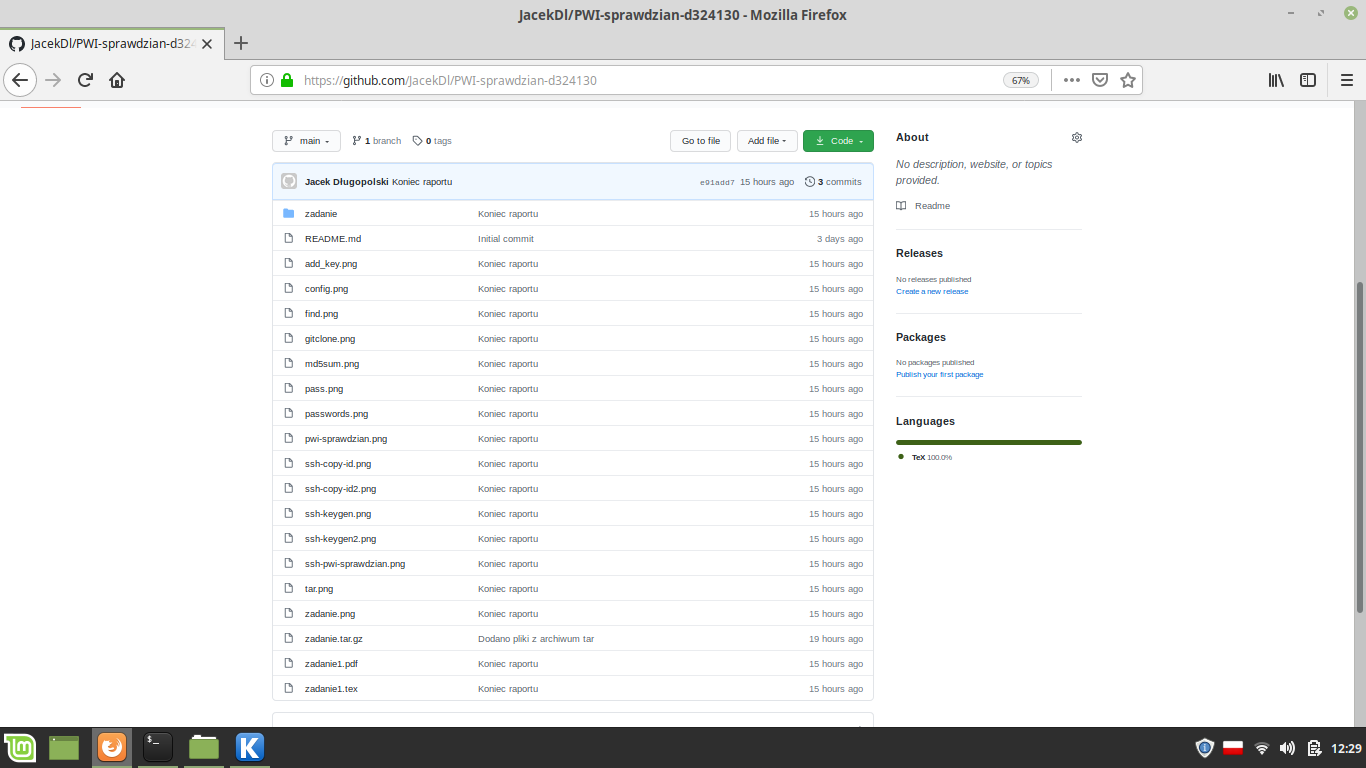
\includegraphics[scale=0.2]{git.png}\\
(z wyjątkiem nazwy ostatniego komita)










 \end{enumerate}
\begin{thebibliography}{6}
    \bibitem{sshcopy}
    man ssh-copy-id
    \bibitem{forward}
    www.cloudsavvit.com/25/what-is-ssh-agent-forwarding-and-how-do-you-use-it/
    \bibitem{tar}
    www.linux.pl/man/index.php?command=tar
	\bibitem{bytefreaks}
	www.bytefreaks.net/gnulinux/creating-an-md5-hash-of-a-string-in-bash
	\bibitem{sed}
	www.geeksforgeeks.org/sed-command-in-linux-unix-with-exaples
	\bibitem{scp}
	www.haydenjames.io/linux-securely-copy-files-using-scp/
    
\end{thebibliography}
 
\end{document}


